\documentclass{article}
\usepackage[margin=1in]{geometry}
\usepackage{hyperref}
\usepackage{multicol}
\usepackage{tikz,tikz-qtree}

\title{CSCI 301, Winter 2017\\Math Exercises \# 5}
\author{Andrew Nguyen}
\date{Due date: }

\begin{document}
\maketitle

Construct a context-free grammar for each of the languages
in questions \ref{cfgbegin} to \ref{cfgend}.
\begin{enumerate}
\item \label{cfgbegin}
$\{0^{2n}1^{n} : n \geq 0\}$

$S \rightarrow \epsilon \mid 00S1$

\item $\{w : w \mbox{ contains at least three 1s}\}$

$S \rightarrow A1A1A1A$	\\
$A \rightarrow \epsilon \mid 0A \mid 1A$

\item $\{w : \mbox{the length of $w$ is odd and its middle symbol is 0}\}$

$S \rightarrow 0S0 \mid 1S1 \mid 0S1 \mid 1S0 \mid 0$

\item $\{w : w \mbox{ is a palindrome}\}$

$S \rightarrow 0S0 \mid 1S1 \mid 0 \mid 1 \mid \epsilon$

\item $\{w : w \mbox{ starts and ends with the same symbol}\}$

$S \rightarrow 0A0 \mid 1A1$ \\
$A \rightarrow \epsilon \mid 0A \mid 1A$

\item  $\{w : w \mbox{ starts and ends with different symbols}\}$

$S \rightarrow 0A1 \mid 1A0$ \\
$A \rightarrow \epsilon \mid 0A \mid 1A$


\item \label{cfgend}
$\{a^mb^n : 0 \leq m \leq n \leq 2m\}$

$S \rightarrow \epsilon \mid ab \mid Sb \mid aaSb$\\
Because of the conditions set on $n$ and $m$: $0 \leq m \leq n \leq 2m$; the number of b's ranges from the number of a's to double the number of a's, and cannot be outside of that range. eg: if there are 5 a's, $aaaaa$, then we must have at least 5 b's but not more than 10 b's. 

$aaaaabbbbb$ fulfills the requisites along with $aaaaabbbbbb$, and $aaaaabbbbbbb$.

So then, for every a we input, we must input at least one b as well. 

\item Let $G$ be the grammar:
\begin{eqnarray*}
S &\rightarrow& aB \mid bA \\
A &\rightarrow& a \mid aS \mid bAA \\
B &\rightarrow& b \mid bS \mid aBB
\end{eqnarray*}
For the string $aaabbabbba$, find a

\begin{enumerate}
\item leftmost derivation,

$S \rightarrow aB$ \\
$aB \rightarrow aaBB$ \\
$aaBB \rightarrow aaaBBB$ \\
$aaaBBB \rightarrow aaabBB$ \\
$aaabBB \rightarrow  aaabbB$ \\
$aaabbB \rightarrow aaabbaBB$ \\
$aaabbaBB \rightarrow  aaabbabB$ \\
$aaabbabB \rightarrow  aaabbabbS$ \\
$aaabbabbS \rightarrow  aaabbabbbA$ \\
$aaabbabbbA \rightarrow  aaabbabbba$ \\

\item rightmost derivation,

$S \rightarrow aB$ \\
$aB \rightarrow aaBB$ \\
$aaBB \rightarrow aaBaBB$ \\
$aaBaBB \rightarrow aaBaBbS$ \\
$aaBaBbS \rightarrow aaBaBbbA$ \\
$aaBaBbbA \rightarrow aaBaBbba$ \\
$aaBaBbba \rightarrow aaBabbba$ \\
$aaBabbba \rightarrow aaaBBabbba$ \\
$aaaBBabbba \rightarrow aaaBbabbba$ \\
$aaaBbabbba \rightarrow aaabbabbba$ \\

\item parse tree.
\item 
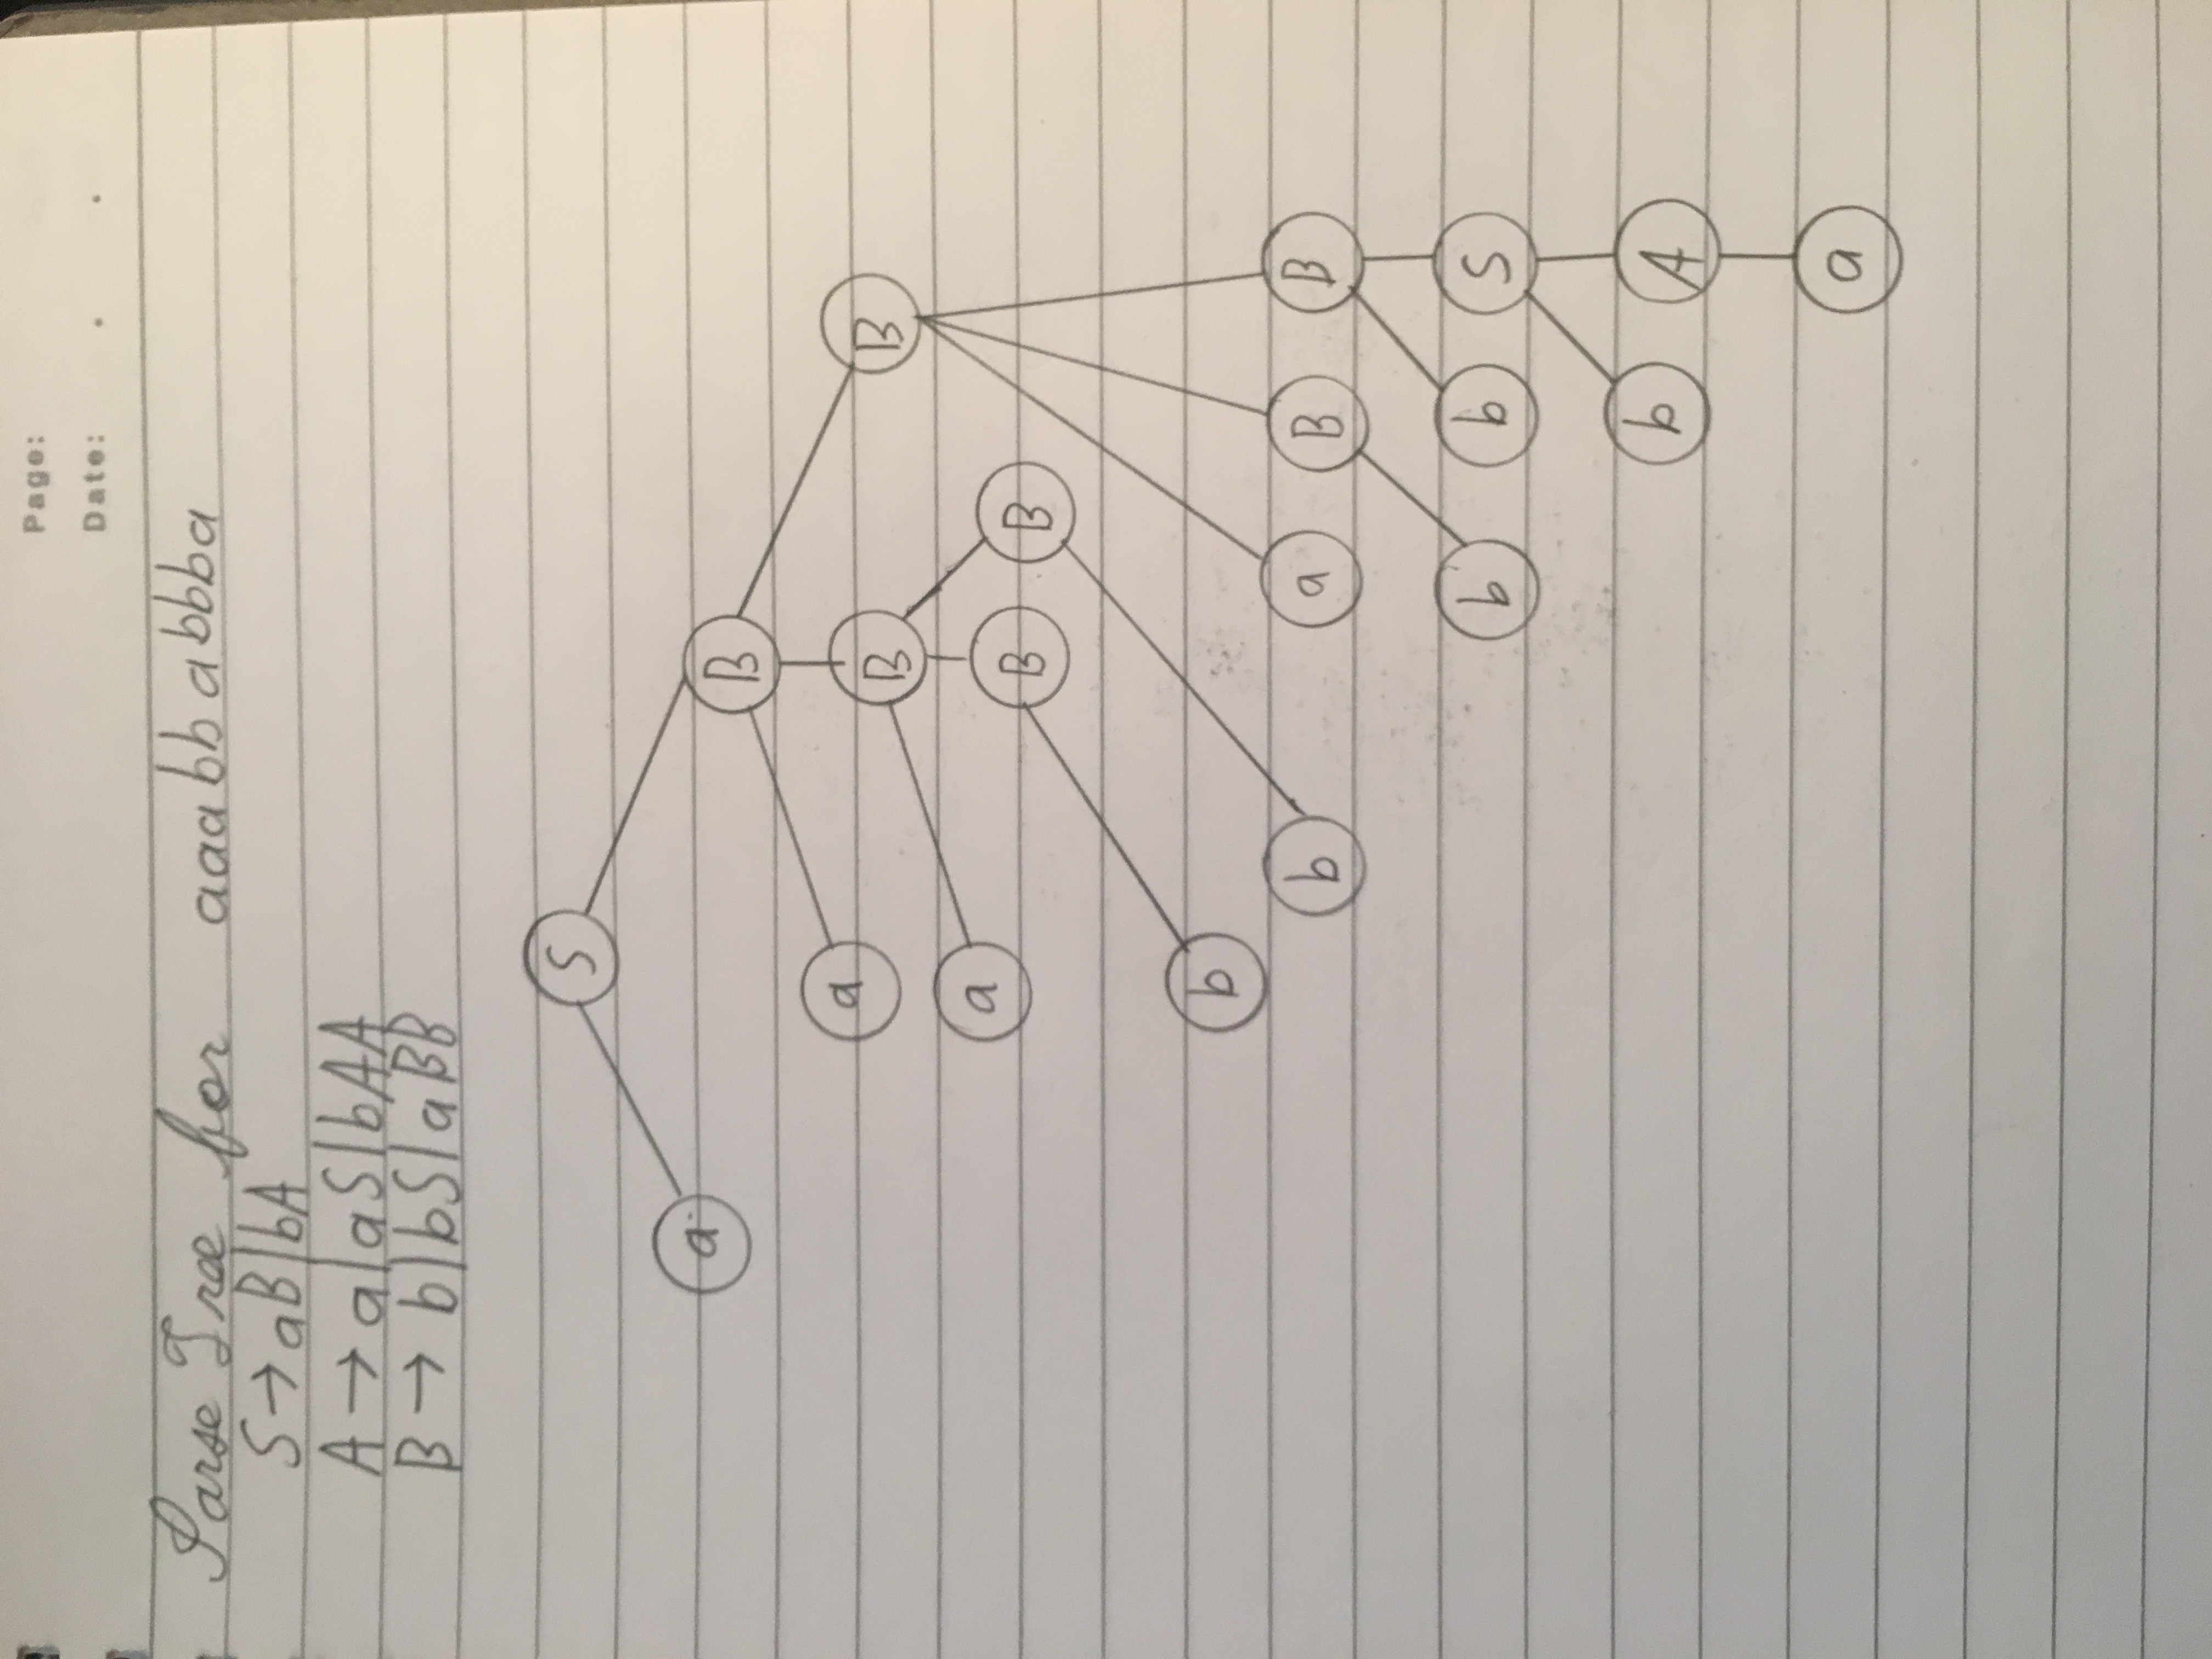
\includegraphics[width=\linewidth]{math05ParseTree}

\end{enumerate}

\item Convert the following grammar to Chomsky normal form:
\begin{eqnarray*}
S &\rightarrow& bA \mid aB\\
A &\rightarrow& bAA \mid aS \mid a\\
B &\rightarrow& aBB \mid bS \mid b
\end{eqnarray*}
Follow the steps documented in my notes
and the text, and show the resulting grammar
after each step.

\begin{description}
\item[Step 1] Eliminate the start variable from the right-hand side of
  rules. 

\item[Step 2] Eliminate $\epsilon$-rules.  

\item[Step 3] Eliminate unit-rules.
  
\item[Step 4] Eliminate all rules having more than two symbols on the
  right-hand side.

\item[Step 5] Eliminate all rules of the form $A\rightarrow u_1u_2$
  where $u_1$ and $u_2$ are not both variables.
  
  $S_0 \rightarrow S$ \\
$S \rightarrow bA \mid aB$ \\
$A \rightarrow bAA \mid aS \mid a$ \\
$B \rightarrow aBB \mid bS \mid b$ \\

$S_0 \rightarrow bA \mid aB$ \\
$S \rightarrow bA \mid aB$ \\
$A \rightarrow bAA \mid abA \mid aaB \mid a$ \\
$B \rightarrow aBB \mid bbA \mid bAB \mid b$ \\

$S_0 \rightarrow S$ \\
$S \rightarrow bA \mid aB$ \\
$A \rightarrow bAA \mid abA \mid aaB \mid a$ \\
$B \rightarrow aBB \mid bbA \mid bAB \mid b$ \\

Introduce new vars\\
$C \rightarrow AA$ \\
$D \rightarrow BB$ \\
$E \rightarrow a$ \\
$F \rightarrow b$ \\
$G \rightarrow ab$ \\
$H \rightarrow ba$ \\
$I \rightarrow aa$ \\
$J \rightarrow bb$ \\

$S_0 \rightarrow S$ \\
$S \rightarrow FA \mid EB$ \\
$A \rightarrow FC \mid GA \mid IB \mid a$ \\
$B \rightarrow ED \mid JA \mid HB \mid b$ \\
$C \rightarrow AA$ \\
$D \rightarrow BB$ \\
$E \rightarrow a$ \\
$F \rightarrow b$ \\
$G \rightarrow ab$ \\
$H \rightarrow ba$ \\
$I \rightarrow aa$ \\
$J \rightarrow bb$ \\

\end{description}
\end{enumerate}
\end{document}